\documentclass[a4paper]{article}
\usepackage[table,xcdraw]{xcolor}
\usepackage[T2A]{fontenc}
\usepackage[utf8]{inputenc}
\usepackage[english, russian]{babel}
\usepackage{graphicx}
\usepackage{epsf,amsbsy,amscd,amsmath,amsfonts,euscript,amssymb,latexsym, textcase, geometry, ifthen, soul}
\usepackage{sbornik}
\geometry{top=2cm}
\geometry{bottom=2cm}
\geometry{left=2cm}
\geometry{right=2cm}
\parindent=1.27cm
\begin{document}
\renewcommand{\refname}{\centering \textnormal {\bf ЛИТЕРАТУРА}}
\renewcommand{\figurename}{Рисунок}
% УДК для Вашей статьи —- обязательно
\noindent{УДК 004.912}
%начало оформление шапки статьи

\begin{center}
%Название Вашей статьи —- {} — обязательное поле; [] необязательное, например, ссылка на грант или благодарность
\ttitle {ИНФОРМАЦИОННЫЕ ОСНОВЫ ВЫДЕЛЕНИЯ АББРЕВИАТУР И\\ИХ РАСШИФРОВКИ В ТЕКСТЕ НА РУССКОМ ЯЗЫКЕ\\Иванов И.И., Петров П.П., Васильев В.В.\\ФГКВОУВО «Академия ФСО России»,\\Россия, Орёл}

\end{center}
%Аннотация и ключевые слова на русском языке
\ruAbstract{Аннотация. Данная работа описывает теоретические основы автоматизированного выделения аббревиатур и определения их расшифровок в текстах на русском языке. Изложено текущее состояние предметной области, рассмотрены существующие программные средства автоматизированного составления списка аббревиатур и их расшифровок. Приводится классификация аббревиатур по структурно-информационным признакам. Предложенная классификация подходит для создания алгоритмов автоматизированного выделения аббревиатур. Разработан подход к определению расшифровки аббревиатур без их непосредственного введения в текст.}

\begin{muquotation}
\small Ключевые слова: аббревиатура, расшифровка аббревиатуры, выделение аббревиатур, классификация аббревиатур.
\end{muquotation}




\quad\textbf{1. Вводные вложения}\\
Развитие аббревиации и использование сокращенных лексических единиц - общая тенденция для многих алфавитных языков. Так, аббревиатуры широко используются не только в специализированных областях знания, но и в повседневной коммуникации [1].

Введ м ряд определений. Под \textit{аббревиатурой} будем понимать слово, образованное сокращением слова или словосочетания, читаемое по названию начальных букв или по начальным и крайним (общепринятые аббревиатуры) звукам слов, входящих в него. Под расшифровкой или полной формой аббревиатуры будем понимать последовательность слов, от которых образована аббревиатура. Введением аббревиатуры в текст является определенная последовательность аббревиатуры и е расшифровки в одном предложении текста. Аббревиатурой без расшифровки является аббревиатура, не имеющая расшифровки в предложении, где она расположена. Под выделением аббревиатуры (расшифровки)будем понимать получение структурной информации об аббревиатуре (расшифровке) для е дальнейшего использования.

Употребление аббревиатур - специфическая особенность научно-технических текстов, в которых аббревиатурам принадлежит большая доля информационной нагрузки [2]. В текстах художественного стиля практически отсутствуют аббревиатуры в виду отсутствия мких терминов, которые необходимо сокращать.

В научно-технических текстах на русском языке из различных областей знаний используются разнообразные аббревиатуры, что затрудняет возможность интуитивной расшифровки аббревиатуры человеком, читающим текст. При отсутствии списка аббревиатур и соответствующих им расшифровок (САиР) для текста возникают трудности с интерпретацией аббревиатур. При этом в большинстве текстов достаточно информации для того, чтобы по определенным признакам восстановить или создать данный список. Это утверждение положено в основу данной статьи. Для отдельных
текстов информации, содержащейся внутри них, может быть недостаточно, чтобы восстановить САиР. Тогда следует прибегать к анализу других текстов схожей тематики.

Потребность в восстановлении САиР может возникнуть при решении широкого класса задач обработки текстов. Здесь можно упомянуть межъязыковые преобразования текстов, в том числе - конверсию графических систем письма [3], расчет характеристик сложности текста [4], автоматизированное извлечение ключевых слов [5], рерайтинг [6] и квалиметрический анализ текста [7]. Во всех перечисленных задачах необходимо произвести предварительное выделение аббревиатур и их расшифровок (ВАиР) из текста.

Исходя из результатов исследования тексты на русском и английском языках можно разделить на три типа (рисунок 1):

1. Тексты, в которых присутствует САиР, введения аббревиатур и аббревиатуры без расшифровок.

2. Тексты, в которых присутствуют введения аббревиатур и аббревиатуры без расшифровок (введ нные ранее).

3. Тексты, которых присутствуют только аббревиатуры без расшифровок (ранее не были введены).

Предполагается, что результаты исследования будут актуальны и для других алфавитных языков. Также установлено, что тексты научно-технического стиля более насыщены аббревиатурами, чем тексты аналогичного объ ма художественного стиля.

\begin{figure}[!h]
\centering
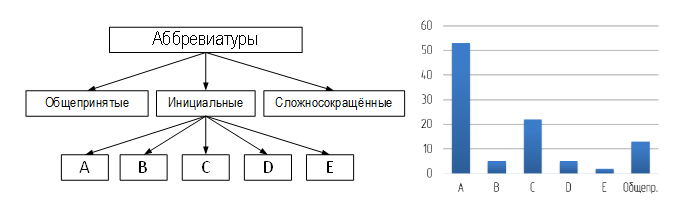
\includegraphics[scale=0.5]{class.png}
\caption{Типы текстов с аббревиатурами (разработано авторами)}
\label{claster_pic1}
\end{figure}

\textbf{2. Состояние предметной области}

В работах [8-10] представляются различные классификации аббревиатур, но не предложено решений по выделению их из текстов.

В работе [11] предложено решение для нахождения полного названия журнала по его аббревиатуре. Неизвестная аббревиатура, указанная пользователем, приводилась в формат регулярного выражения, которое предполагало возможный набор слов, начинающийся с указанных букв. Специфическая реализация полученного решения не позволяет использовать его для определения полных форм аббревиатур из других предметных областей.

В работах [12, 13] на основании определения частот встречаемости соседних слов определяется мера их связности, что позволяет предложить вероятные полные формы аббревиатур. Достоинством такого метода является его универсальность, недостатком - высокая трудо мкость. Материалы данных работ использовались при разработке модели процесса выделения аббревиатур.

В работах [14, 15] предложено исходный текст представлять в виде совокупности тем, которые образуются множеством входящих в них с разной вероятностью слов. Найденная схожесть частей текста используется как представление полной формы аббревиатуры. Данных подход предлагает множество решений с близкими вероятностями, что предусматривает дополнительную работу для пользователя на стадии отбора расшифровки интересующей аббревиатуры.

Существуют программы для ЭВМ, зарегистрированные в Федеральной службе по интеллектуальной собственности (Роспатент), обладающие возможностью выявления САиР. Так, программа [16] реализует функцию автоматизированного формирования перечня аббревиатур, решает задачу формирования единой базы терминов (аббревиатур) и их определений (расшифровок). Программа [17] предназначена для автоматизированного извлечения терминологических структур из монографии заданной предметной области. Одной из основных функций программы является извлечение терминов, в частности, расшифровка аббревиатур.

3. Классификация аббревиатур

Формирование классификации аббревиатур осложнено особенностями их структуры, большой вариативностью, множеством различных способов аббревиации, а также взаимодействием аббревиации с другими способами словообразования. Исследователи [10, 18, 19] сходятся во мнении, что аббревиатуры можно подразделять на инициальные, сложносокращ нные и общепринятые. В первом случае аббревиатура составляется из первых букв е расшифровки. Во втором случае в аббревиатуру включены не только первые, но и другие буквы сокращаемых слов [20]. В третьем случае аббревиатуры имеют уникальное представление в тексте и единственную расшифровку. Общепринятые аббревиатуры, как правило, интуитивно
понятны и употребляются перед определ нными структурами в тексте.

Для решения задачи автоматизированного ВАиР из текста введ м классификацию по структурно-информационным признакам, а также приведем в первом приближении их распространенность, изученную на материале ста случайно отобранных статей с ресурса Cyberleninka.ru. Аббревиатуры разделяются на три класса: инициальные, общепринятые и сложносокращ нные. Инициальные и общепринятые аббревиатуры имеют выраженную структуру (прописные буквы, знаки препинания), которой сложносокращ нные не обладают (структурный признак). При этом, общепринятые аббревиатуры имеют интуитивно понятный смысл, а инициальные требуют расшифровки в тексте (информационный признак). Сложносокращ нные аббревиатуры, не имеющие в составе прописных букв (завхоз, ликбез и т.д.), рассматриваться в данной статье не будут. Инициальные аббревиатуры разделены на пять типов, каждый из которых отличается по структурным признакам (рисунок 2).\\

\begin{figure}[!h]
\centering
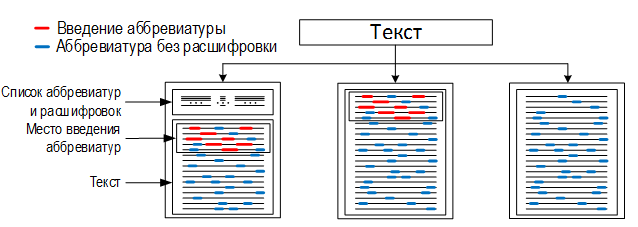
\includegraphics[scale=0.8]{abr.png}
\caption{Классификация аббревиатур по структурно-информационным признакам (разработано авторами)}
\label{claster_pic1}
\end{figure}

Для создания программного средства ВАиР необходимо учитывать особенности каждого класса рассматриваемых аббревиатур.

Особенности инициальных и общепринятых аббревиатур:

1. (тип А, 53\%) Инициальная аббревиатура, в которой слова полной формы разделены только пробелами и в не входят только первые буквы слов полной формы. Например: центр информационной безопасности (ЦИБ), Latent Dirichlet Allocation (LDA).

2. (тип B, 5\%) Инициальная аббревиатура, в которой некоторые слова полной формы объединены знаком дефис или символом «косой черты». Например: оптико-тепловизионный комплекс (ОТК), read-only memory (ROM), input/output (IO).

3. (тип C, 22\%) Инициальная аббревиатура с элементами сложносокращ нных слов. При этом, аббревиатура может состоять не только из прописных букв, но первая буква полной формы должна соответствовать первой букве аббревиатуры. Количество слов в расшифровке не совпадает с количеством букв в аббревиатуре. Например: гидрометеорологическая станция (ГМС), ammonium bifluoride (ABF), Белорусский автомобильный завод (БелАЗ), временно исполняющий обязанности (ВрИО).

4. (тип D, 5\%) Инициальная аббревиатура, отличная от языка документа. Например, протокол передачи файлов (FTP), временный идентификационный номер подвижного абонента (TMSI).

5. (тип E, 2\%) Инициальная аббревиатура, в которой буквы аббревиатуры разделены точками, а первые буквы слов полной формы соответствуют буквам в аббревиатуре. Например: Фамилия Имя Отчество (Ф.И.О.), Петроградская сторона (П.С.).

6. Общепринятые аббревиатуры (13\%), которые применяются в разных областях: адреса (г., ул., д., пр-т), звания (к-т, л-т), точные науки (см, Гц), время суток (a.m, p.m), элемент текста (P.S.) и т.п. Они не имеют полной формы в тексте и будут расшифровываться по словарю.

Для примеров были использованы аббревиатуры на русском и английском языках, но предполагается, что данная классификация актуальна и для других алфавитных языков.

\textbf{4. Модель процесса выделения аббревиатур и расшифровок из текста}

Процесс выделения аббревиатур и их расшифровок в общем может состоять из двух этапов.

\textbf{Первый этап} заключается в разделении исходного текста на предложения. Он необходим для более точного определения расшифровок аббревиатур. Разделителем предложений в тексте могут являться восклицательные и вопросительные знаки, многоточия, знаки переноса строки и точки. Однако возникает ряд проблем, связанных с тем, что точки ставятся в тексте не только в конце предложения. Чаще всего точки можно встретить в следующих конструкциях: в датах (25.10.20 г.), в адресах (ул. Ленина, д. 7), в общих аббревиатурах (т.д.), в буквенно-цифровых обозначениях (66.КП.ВРБ.00.00.00.ВО), перед номерами телефонов (тел. 89997773737), в нумерации (1.1, 1.2, 1.3), в составе сокращения ФИО (А.А. Иванов) и в инициальных аббревиатурах (R.I.S.K.).

\textbf{Второй этап} разбивается на две параллельных части: \textit{поиск мест
введения аббревиатур} и \textit{поиск аббревиатур без расшифровок} в предложениях.

\textit{Поиск мест введения аббревиатур} заключается в анализе предложения на предмет наличия аббревиатуры и соответствующей расшифровки. В случае успеха информация о расшифровке и соответствующей аббревиатуре заносится в базу данных. Одна аббревиатура вводится в тексте только один раз.

\textit{Введения аббревиатур} имеют определенную структуру, которая задается формулой (таблица 1) [3]. Возможны ситуации, когда при введении аббревиатуры в скобках может присутствовать текст, который не относится ни к расшифровке, ни к аббревиатуре.


Таблица 1. Типовые формулы введения аббревиатур

\begin{table}[h]\begin{center}
\scalebox{0.9}{

\begin{tabular}{|c|c|}

\hline
\rowcolor[HTML]{C0C0C0}
{\color[HTML]{000000} \textbf{Формула введения}} & \textbf{Примеры} \\ \hline
\multicolumn{1}{|l|}{расшифровка (аббревиатура)} & \begin{tabular}[c]{@{}c@{}}Специальное программное обеспечение (СПО),\\ система (С)\end{tabular} \\ \hline
аббревиатура (расшифровка) & \begin{tabular}[c]{@{}c@{}}АС (автоматическая сигнализация), СО (сигнал\\ ожидания)\end{tabular} \\ \hline
расшифровка аббревиатура & \begin{tabular}[c]{@{}c@{}}Процессор преобразования матриц ППМ,\\ двухпроцессорная система ДС\end{tabular} \\ \hline
аббревиатура - расшифровка & \begin{tabular}[c]{@{}c@{}}ЯМД - язык манипулирования данными, ЯУ - язык\\ управления\end{tabular} \\ \hline
расшифровка - аббревиатура & \begin{tabular}[c]{@{}c@{}}Главная машина - ГМ\end{tabular} \\ \hline

\end{tabular}}
\end{center}
\end{table}


Поиск аббревиатур без расшифровок заключается в определении по определенным признакам наличия аббревиатур в предложении.

В процессе поиска могут встречаться аббревиатуры, которые ранее не были введены в тексте. В связи с этим появляется необходимость поиска информации об их расшифровках по другим источникам. Для корректного сопоставления аббревиатуры и расшифровки из разных текстов, необходимо учитывать контекст аббревиатур (рисунок 3). \\
\begin{figure}[!h]
\centering
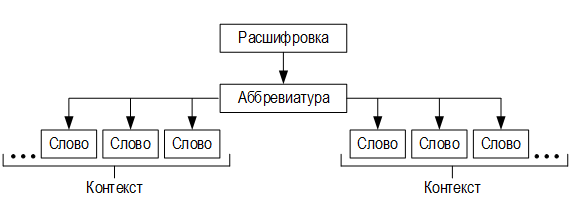
\includegraphics[scale=0.8]{rash.PNG}
\caption{Соответствие расшифровки, аббревиатуры и контекста (разработано авторами}
\label{claster_pic1}
\end{figure}

Так как одна аббревиатура вводится в тексте, как правило, только один раз, то далее по тексту будут встречаться только аббревиатуры без расшифровок, при этом каждая выделенная аббревиатура будет однозначно соответствовать введенной ранее. Далее от предложения к предложению необходимо считывать аббревиатуры и их контекст в базу данных, после чего производить сопоставление с информацией, полученной при поиске мест введения \textit{аббревиатур}. В случае отсутствия расшифровок необходимо производить поиск по другим текстам или по словарю.

Принципиальная схема ВАиР в тексте приведена на рисунке 4.\\
\begin{figure}[!h]
\centering
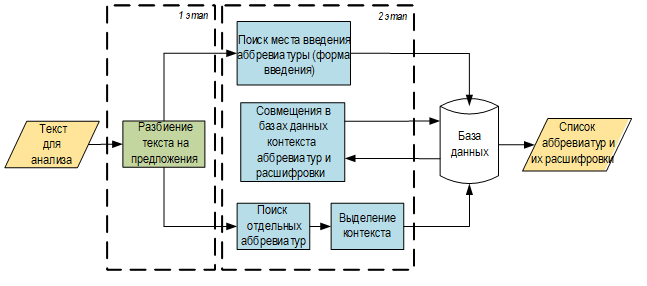
\includegraphics[scale=0.8]{prin.png}
\caption{- Принципиальная схема выделения аббревиатур и
расшифровок в тексте (разработано авторами)}
\label{claster_pic1}
\end{figure}


\textbf{5. Заключение}
В статье рассматривается обобщенное гиперболическое уравнение запаздывающего типа с некарлемановскими сдвигами вида

$$U_{xx}(x,y)-U_{yy}(x,y)=H(x-\tau)[U_x (x-\tau,y)+U(x-\tau,y)],\eqno (1)$$
$0 < \tau\equiv const, H(\epsilon) - \text{функция Хевисайд; в области}$
$$ D=\{(x,y): x> 0,y<0\}=U_{k=0}^\infty D_k,$$
где\\
$D_k=\{(x,y):k\tau - y \leq x \leq (k+1)\tau +y,\frac{\tau}{2}<y<0\}\text{ }(k=0,1,2, ...).$

\textbf{Задача К.} Найти в области D решение уравнения 1 из класса $C(\bar D)\cap C^2(D)$, удоволетворяющее условиям

$$U(x,y)|_{y=0} = \omega(x),x \geq 0 \text{,}\eqno(2)$$
$$U_y(x,y)|_{y=0}=v(x),x>0 \text{,}\eqno(3)$$
где $\omega(X)$,$v(x)$ - заданные непрерывные достаточно гладкие функции, причем $\omega(0)=\omega(+\infty)=0$.
\begin{center}
\textbf{Список литературы}
\end{center}

1. Максименко, О.И. Новые тенденции аббревиации (на материале русского, английского и немецкого языков) // Вестник
Российского университета дружбы народов. Серия: Теория языка. Семиотика. Семантика. – 2017. – Т. 8. – № 1. – С. 174-181.

2. Грязнухина, Т.А. Лингвистические проблемы автоматизации редакционно-издательских процессов / Т.А. Грязнухина, Н.П. Дарчук, Л.И. Комарова и др.; отв. ред. В.И. Перебейнос, М.Д. Феллер // колл. монография: Академия наук УССР, Институт языковедения им. А.А. Потебни. — Киев: Наукова думка, 1986. – 229 с.

3. Гращенко, Л.А. Информационные основы польско-русского межъязыкового преобразования текстов / Л.А. Гращенко, Н.Н. Пивоваров // Новые информационные технологии в автоматизированных системах. – 2016. – № 19. – С. 101-106.


4. Мизернов, И.Ю. Анализ методов оценки сложности текста / И.Ю. Мизернов, Л.А. Гращенко // Новые информационные технологии в автоматизированных системах. – 2015. – № 18. – С. 572-581.

5. Ванюшкин, А.С. Методы и алгоритмы извлечения ключевых слов / А.С. Ванюшкин, Л.А. Гращенко // Новые информационные технологии в автоматизированных системах. – 2016. – № 19. – С. 85-93.

6. Науменко, Д.А. Информационные основы автоматизации рерайтинга / Д.А. Науменко, Л.А. Гращенко, Г.В. Романишин // Новые информационные технологии в автоматизированных системах. – 2019. – № 22. – С. 187-191.

7. Гращенко, Л.А. Опыт автоматизированного анализа повторов в научных текстах / Л.А. Гращенко, Г.В. Романишин // Новые информационные технологии в автоматизированных системах. – 2015. – № 18. – С. 582-590.

8. Суперанская, А.В. Общая терминология: Вопросы теории. Аббревиация в терминологии / А.В. Суперанская, Н.В. Подольская, Н.В. Васильева. – Изд. 6-е. – М.: Книжный дом «ЛИБРОКОМ», 2012. – 248 с.

9. Нургалеева, Т.Г. Аббревиация как средство экспрессивного словообразования: автореф. дис. канд. филол. наук, спец. 10.02.04 «Германские языки» / Т. Г. Нургалеева. — М.: Наука, 2010. — 240 с.
10. Земская, Е.А. Современный русский язык. Словообразование: учеб. Пособие. 3-е изд., испр. и доб. – М.: Наука, 2011.

11. Jenkins K. Deciphering Journal Abbreviations with JAbbr // Code4Lib Journal. – 2009. – № 7. [Электронный ресурс] URL:https://journal.code4lib.org/articles/1758 (Дата обращения: 09.11.2021)

12. Mikolov T. Efficient Estimation of Word Representations in Vector Space / T. Mikolov, K. Chen, G. Corrado, J. Dean // arXiv.org. — 2013. [Электронный ресурс] URL:http://arxiv.org/pdf/1301.3781v3.pdf (Дата обращения: 10.11.2021)
13. Mikolov T. Distributed Representations of Words and Phrases and their Compositionality / T. Mikolov, I. Sutskever, K. Chen, G. Corrado, J. Dean // Advances in Neural Information Processing Systems. – 2013. – P. 3111-3119.

14. Blei, D.M. Latent Dirichlet Allocation / D.M. Blei, A.Y. Ng, M.I. Jordan // Journal of Machine Learning Research. – 2003. – № 3. – P. 993-1022.

15. Heinrich G. Parameter estimation for text analysis. — 2004. [Электронный ресурс] URL:http://citeseerx.ist.psu.edu/view-doc/summary?doi=10... (Дата обращения: 10.11.2021)

16. Автоматизированное формирование перечня аббревиатур (сокращений) / А.А. Чумичкин, М.В. Рутц, Г.И. Трифонов // Свидетельство о регистрации программы для ЭВМ RU 2018663069, 19.10.2018. Заявка № 2018660897 от 04.10.2018.

17. Программа для извлечения и анализа терминологических структур смежных предметных областей / Д.А. Губанов // Свидетельство о регистрации программы для ЭВМ RU 2019665358, 22.11.2019. Заявка № 2018664640 от 18.11.2019.

18. Алексеев, Д.И. Сокращ нные слова в русском языке. – Саратов: Изд-во Саратовского ун-та, 1979. – 328 с.

19. Виноградова, В.В. Русская грамматика: научные труды. В 2 т. Т. 1 – М.: Российская академия наук, 2005. — 784 с.

20. Ахманова, О.С. Словарь лингвистических терминов. – М.: Едиториа УРСС, 2004. – 576 с.
\end{document}